\documentclass[12pt,a4paper]{article}
\usepackage[utf8]{vietnam}
\usepackage{amsmath,amssymb}
\usepackage[a4paper,left=2cm,right=1.8cm,top=1.8cm,bottom=1.8cm]{geometry}
\usepackage{tikz}
\usepackage{array,tabularx,longtable}
\usepackage{enumitem}
\setlength{\parindent}{0pt}
\setlength{\parskip}{3pt}
\linespread{1.15}
\pagestyle{plain}

% Phương án trắc nghiệm: 4 phương án trên 1 dòng / 2 dòng / mỗi phương án 1 dòng
\newcommand{\bonpa}[4]{\par\noindent\begin{tabularx}{\linewidth}{@{\hspace{0.6cm}}XXXX@{}}
\textbf{A.} #1 & \textbf{B.} #2 & \textbf{C.} #3 & \textbf{D.} #4\end{tabularx}\par}
\newcommand{\haipa}[4]{\par\noindent\begin{tabularx}{\linewidth}{@{\hspace{0.6cm}}XX@{}}
\textbf{A.} #1 & \textbf{B.} #2\\ \textbf{C.} #3 & \textbf{D.} #4\end{tabularx}\par}
\newcommand{\motpa}[4]{\par\hspace*{0.6cm}\textbf{A.} #1\par\hspace*{0.6cm}\textbf{B.} #2\par
\hspace*{0.6cm}\textbf{C.} #3\par\hspace*{0.6cm}\textbf{D.} #4\par}
\newcommand{\cau}[1]{\par\medskip\textbf{Câu #1.}~}
\newcommand{\bai}[2]{\par\medskip\textbf{Bài #1} \textit{(#2)}.~}
\newcommand{\y}[1]{\par\hspace*{0.6cm}#1}
\newcommand{\phan}[1]{\par\bigskip{\large\textbf{#1}}\par\smallskip}
\setlength{\extrarowheight}{2pt}

\begin{document}
% ===================== ĐỀ SỐ 4 =====================
\noindent
\begin{minipage}[t]{0.38\linewidth}\centering
TRƯỜNG THCS \dotfill\\[2pt]
\textbf{ĐỀ SỐ 4}
\end{minipage}\hfill
\begin{minipage}[t]{0.6\linewidth}\centering
\textbf{ĐỀ KIỂM TRA GIỮA HỌC KÌ I}\\
\textbf{NĂM HỌC 2026 -- 2027}\\
\textbf{MÔN: TOÁN 7} -- Sách \textit{Kết nối tri thức với cuộc sống}\\
\textit{Thời gian làm bài: 90 phút (không kể thời gian giao đề)}
\end{minipage}

\medskip
Họ và tên: \dotfill\ Lớp: \makebox[2cm]{\dotfill}\ Số báo danh: \makebox[2.5cm]{\dotfill}
\phan{A. TRẮC NGHIỆM (3,0 điểm)}
\textbf{Phần I. Câu trắc nghiệm nhiều phương án lựa chọn} \textit{(1,0 điểm)}. Thí sinh trả lời từ câu 1 đến câu 4. Mỗi câu hỏi thí sinh chỉ chọn một phương án.
\cau{1} Cách viết nào sau đây là đúng?
\bonpa{$-\dfrac{2}{3}\in\mathbb{N}$}{$-5\notin\mathbb{Q}$}{$\dfrac{1}{2}\in\mathbb{Z}$}{$-0{,}4\in\mathbb{Q}$}
\cau{2} Kết quả của phép tính $\left(3^{2}\right)^{4}$ là
\bonpa{$3^{6}$}{$3^{8}$}{$3^{16}$}{$9^{8}$}
\cau{3} Phân số nào sau đây viết được dưới dạng số thập phân hữu hạn?
\bonpa{$\dfrac{1}{6}$}{$\dfrac{2}{15}$}{$\dfrac{7}{40}$}{$\dfrac{5}{9}$}
\cau{4} Qua một điểm nằm ngoài một đường thẳng, có bao nhiêu đường thẳng song song với đường thẳng đó?
\bonpa{Không có.}{Chỉ có một.}{Có hai.}{Có vô số.}

\medskip\textbf{Phần II. Câu trắc nghiệm đúng sai} \textit{(1,0 điểm)}. Trong mỗi ý a), b), c), d) ở câu 5, thí sinh chọn đúng hoặc sai.
\cau{5} Cho tam giác $ABC$ có $\widehat{A}=60^\circ$ và $\widehat{B}=2\widehat{C}$.
\y{a) $\widehat{B}=60^\circ$.}
\y{b) $\widehat{B}+\widehat{C}=120^\circ$.}
\y{c) Tam giác $ABC$ là tam giác tù.}
\y{d) $\widehat{C}=40^\circ$.}

\medskip\textbf{Phần III. Câu trắc nghiệm trả lời ngắn} \textit{(1,0 điểm)}. Thí sinh trả lời từ câu 6 đến câu 9.
\cau{6} Tính $1{,}5+\left(-\dfrac{3}{4}\right)$ (viết kết quả dưới dạng số thập phân).
\cau{7} Tìm $x$, biết $2x+\dfrac{1}{2}=\dfrac{9}{2}$.
\cau{8} Tính giá trị của biểu thức $\dfrac{4^{5}}{2^{8}}$.
\cau{9} Cho $\widehat{xOy}$ và $\widehat{yOx'}$ là hai góc kề bù, $\widehat{xOy}=110^\circ$. Tia $Ot$ là tia phân giác của $\widehat{yOx'}$. Tính số đo $\widehat{tOx'}$ (đơn vị: độ).
\phan{B. TỰ LUẬN (7,0 điểm)}
\bai{1}{1,0 điểm} Tính (hợp lí nếu có thể):
\y{a) $25\cdot\left(-\dfrac{1}{5}\right)^{3}+\dfrac{1}{5}-2\cdot\left(-\dfrac{1}{2}\right)^{2}$;}
\y{b) $\dfrac{3}{5}:\left(-\dfrac{1}{15}-\dfrac{1}{6}\right)+\dfrac{3}{5}:\left(-\dfrac{1}{3}-\dfrac{16}{15}\right)$.}
\bai{2}{1,5 điểm} Tìm $x$, biết:
\y{a) $-\dfrac{5}{6}+x=\dfrac{1}{4}$;}
\y{b) $\left(x+\dfrac{1}{5}\right):\dfrac{3}{4}=-\dfrac{2}{3}$;}
\y{c) $3^{x-1}+5\cdot 3^{x-1}=162$.}
\bai{3}{1,0 điểm} Một chiếc áo có giá niêm yết là $250\,000$ đồng. Nhân dịp khai trương, cửa hàng giảm giá $\dfrac{1}{5}$ giá niêm yết. Riêng khách hàng có thẻ thành viên được giảm thêm $\dfrac{1}{10}$ giá đã giảm. Bạn An có thẻ thành viên, hỏi bạn An phải trả bao nhiêu tiền để mua chiếc áo đó?
\bai{4}{1,5 điểm} Cho hình vẽ bên, tam giác $ABC$ có $\widehat{B}=60^\circ$, $\widehat{C}=45^\circ$; đường thẳng $a$ đi qua $A$ và song song với $BC$.
\begin{center}
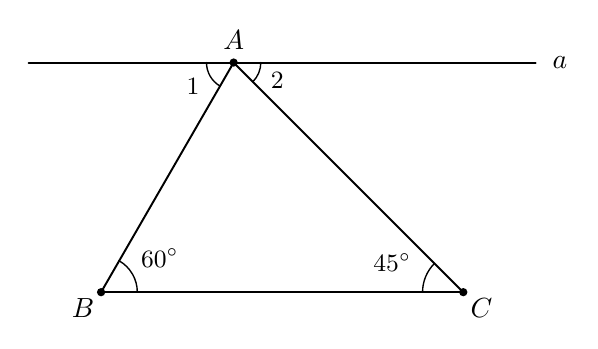
\begin{tikzpicture}[scale=1.15,line cap=round,line join=round]
  \draw[line width=0.7pt] (1.464,2.536) -- (0.000,0.000);
  \draw[line width=0.7pt] (0.000,0.000) -- (4.000,0.000);
  \draw[line width=0.7pt] (4.000,0.000) -- (1.464,2.536);
  \draw[line width=0.7pt] (-0.800,2.536) -- (4.800,2.536);
  \node[anchor=west,inner sep=1pt] at (4.950,2.536) {$a$};
  \fill (1.464,2.536) circle (1.3pt);
  \node[anchor=center,inner sep=1pt] at (1.464,2.786) {$A$};
  \fill (0.000,0.000) circle (1.3pt);
  \node[anchor=center,inner sep=1pt] at (-0.200,-0.180) {$B$};
  \fill (4.000,0.000) circle (1.3pt);
  \node[anchor=center,inner sep=1pt] at (4.200,-0.180) {$C$};
  \draw[line width=0.5pt] (0.400,0.000) arc[start angle=0,end angle=60,radius=0.400];
  \node[anchor=center,inner sep=1pt] at (0.650,0.375) {{\small $60^\circ$}};
  \draw[line width=0.5pt] (3.682,0.318) arc[start angle=135,end angle=180,radius=0.450];
  \node[anchor=center,inner sep=1pt] at (3.215,0.325) {{\small $45^\circ$}};
  \draw[line width=0.5pt] (1.164,2.536) arc[start angle=180,end angle=240,radius=0.300];
  \node[anchor=center,inner sep=1pt] at (1.014,2.276) {{\small 1}};
  \draw[line width=0.5pt] (1.676,2.324) arc[start angle=315,end angle=360,radius=0.300];
  \node[anchor=center,inner sep=1pt] at (1.945,2.337) {{\small 2}};
\end{tikzpicture}
\end{center}
\y{a) Tính số đo $\widehat{A_1}$.}
\y{b) Tính số đo $\widehat{A_2}$.}
\y{c) Tính số đo $\widehat{BAC}$.}
\bai{5}{1,5 điểm} Cho tứ giác $ABCD$ có $AB=CD$ và $AD=BC$ (như hình vẽ dưới đây).
\begin{center}
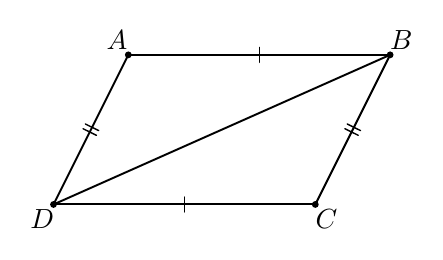
\begin{tikzpicture}[scale=0.95,line cap=round,line join=round]
  \draw[line width=0.7pt] (1.000,2.000) -- (4.500,2.000);
  \draw[line width=0.7pt] (4.500,2.000) -- (3.500,0.000);
  \draw[line width=0.7pt] (3.500,0.000) -- (0.000,0.000);
  \draw[line width=0.7pt] (0.000,0.000) -- (1.000,2.000);
  \draw[line width=0.7pt] (4.500,2.000) -- (0.000,0.000);
  \draw[line width=0.5pt] (2.750,1.900) -- (2.750,2.100);
  \draw[line width=0.5pt] (1.750,-0.100) -- (1.750,0.100);
  \draw[line width=0.5pt] (0.426,1.076) -- (0.605,0.987);
  \draw[line width=0.5pt] (0.395,1.013) -- (0.574,0.924);
  \draw[line width=0.5pt] (3.926,1.076) -- (4.105,0.987);
  \draw[line width=0.5pt] (3.895,1.013) -- (4.074,0.924);
  \fill (1.000,2.000) circle (1.3pt);
  \node[anchor=center,inner sep=1pt] at (0.850,2.200) {$A$};
  \fill (4.500,2.000) circle (1.3pt);
  \node[anchor=center,inner sep=1pt] at (4.650,2.200) {$B$};
  \fill (3.500,0.000) circle (1.3pt);
  \node[anchor=center,inner sep=1pt] at (3.650,-0.200) {$C$};
  \fill (0.000,0.000) circle (1.3pt);
  \node[anchor=center,inner sep=1pt] at (-0.150,-0.200) {$D$};
\end{tikzpicture}
\end{center}
\y{a) Chứng minh $\triangle ABD=\triangle CDB$.}
\y{b) Chứng minh $AB\parallel CD$.}
\y{c) Chứng minh $AD\parallel BC$.}
\bai{6}{0,5 điểm} Tính tổng $B=1+\dfrac{1}{2}+\dfrac{1}{2^{2}}+\dfrac{1}{2^{3}}+\ldots+\dfrac{1}{2^{100}}$.

\bigskip\begin{center}\textbf{--------- HẾT ---------}\\
\textit{Giáo viên coi kiểm tra không giải thích gì thêm.}\end{center}

\newpage
\begin{center}{\large\textbf{HƯỚNG DẪN CHẤM -- ĐỀ SỐ 4}}\end{center}
\phan{A. TRẮC NGHIỆM (3,0 điểm)}
\textbf{Phần I.} Mỗi câu trả lời đúng được 0,25 điểm.

\begin{tabular}{|l|*{4}{>{\centering\arraybackslash}p{2cm}|}}\hline
Câu & 1 & 2 & 3 & 4 \\ \hline
Đáp án & \textbf{D} & \textbf{B} & \textbf{C} & \textbf{B} \\ \hline
\end{tabular}

\textbf{Phần II.} Mỗi ý trả lời đúng được 0,25 điểm.

\begin{tabular}{|l|*{4}{>{\centering\arraybackslash}p{2cm}|}}\hline
Câu 5 & a) & b) & c) & d) \\ \hline
Đáp án & \textbf{Sai} & \textbf{Đúng} & \textbf{Sai} & \textbf{Đúng} \\ \hline
\end{tabular}

\textbf{Phần III.} Mỗi câu trả lời đúng được 0,25 điểm.

\begin{tabular}{|l|*{4}{>{\centering\arraybackslash}p{2cm}|}}\hline
Câu & 6 & 7 & 8 & 9 \\ \hline
Đáp án & \textbf{0,75} & \textbf{2} & \textbf{4} & \textbf{35} \\ \hline
\end{tabular}

\phan{B. TỰ LUẬN (7,0 điểm)}
\begin{longtable}{|>{\bfseries}c|p{0.76\linewidth}|>{\centering\arraybackslash}p{1.3cm}|}\hline
Bài & \multicolumn{1}{c|}{\textbf{Nội dung}} & \textbf{Điểm} \\ \hline\endhead
1a & \rule{0pt}{4ex}$=25\cdot\left(-\dfrac{1}{125}\right)+\dfrac{1}{5}-2\cdot\dfrac{1}{4}=-\dfrac{1}{5}+\dfrac{1}{5}-\dfrac{1}{2}$\rule[-2.4ex]{0pt}{0pt} & 0,25 \\ \hline
 & \rule{0pt}{4ex}$=-\dfrac{1}{2}$\rule[-2.4ex]{0pt}{0pt} & 0,25 \\ \hline
1b & \rule{0pt}{4ex}$=\dfrac{3}{5}:\left(-\dfrac{7}{30}\right)+\dfrac{3}{5}:\left(-\dfrac{7}{5}\right)=-\dfrac{18}{7}+\left(-\dfrac{3}{7}\right)$\rule[-2.4ex]{0pt}{0pt} & 0,25 \\ \hline
 & \rule{0pt}{4ex}$=-\dfrac{21}{7}=-3$\rule[-2.4ex]{0pt}{0pt} & 0,25 \\ \hline
2a & \rule{0pt}{4ex}$x=\dfrac{1}{4}+\dfrac{5}{6}=\dfrac{3}{12}+\dfrac{10}{12}$\rule[-2.4ex]{0pt}{0pt} & 0,25 \\ \hline
 & \rule{0pt}{4ex}$x=\dfrac{13}{12}$. Vậy $x=\dfrac{13}{12}$.\rule[-2.4ex]{0pt}{0pt} & 0,25 \\ \hline
2b & \rule{0pt}{4ex}$x+\dfrac{1}{5}=-\dfrac{2}{3}\cdot\dfrac{3}{4}=-\dfrac{1}{2}$\rule[-2.4ex]{0pt}{0pt} & 0,25 \\ \hline
 & \rule{0pt}{4ex}$x=-\dfrac{1}{2}-\dfrac{1}{5}=-\dfrac{7}{10}$. Vậy $x=-\dfrac{7}{10}$.\rule[-2.4ex]{0pt}{0pt} & 0,25 \\ \hline
2c & $3^{x-1}\cdot(1+5)=162$, suy ra $3^{x-1}=27=3^{3}$ & 0,25 \\ \hline
 & $x-1=3$, $x=4$. Vậy $x=4$. & 0,25 \\ \hline
3 & \rule{0pt}{4ex}Số tiền được giảm lần thứ nhất: $250\,000\cdot\dfrac{1}{5}=50\,000$ (đồng).\rule[-2.4ex]{0pt}{0pt} & 0,25 \\ \hline
 & Giá chiếc áo sau khi giảm lần thứ nhất: $250\,000-50\,000=200\,000$ (đồng). & 0,25 \\ \hline
 & \rule{0pt}{4ex}Số tiền bạn An được giảm thêm: $200\,000\cdot\dfrac{1}{10}=20\,000$ (đồng).\rule[-2.4ex]{0pt}{0pt} & 0,25 \\ \hline
 & Số tiền bạn An phải trả: $200\,000-20\,000=180\,000$ (đồng). & 0,25 \\ \hline
4a & Vì $a\parallel BC$ nên $\widehat{A_1}=\widehat{B}$ (hai góc so le trong) & 0,25 \\ \hline
 & Do đó $\widehat{A_1}=60^\circ$. & 0,25 \\ \hline
4b & Vì $a\parallel BC$ nên $\widehat{A_2}=\widehat{C}$ (hai góc so le trong) & 0,25 \\ \hline
 & Do đó $\widehat{A_2}=45^\circ$. & 0,25 \\ \hline
4c & Ta có $\widehat{A_1}+\widehat{BAC}+\widehat{A_2}=180^\circ$ & 0,25 \\ \hline
 & nên $\widehat{BAC}=180^\circ-60^\circ-45^\circ=75^\circ$. & 0,25 \\ \hline
5 & Ghi GT – KL đúng. & 0,25 \\ \hline
5a & Xét $\triangle ABD$ và $\triangle CDB$ có: $AB=CD$ (gt); $AD=CB$ (gt); $BD$ là cạnh chung. & 0,25 \\ \hline
 & Do đó $\triangle ABD=\triangle CDB$ (c.c.c). & 0,25 \\ \hline
5b & Từ câu a suy ra $\widehat{ABD}=\widehat{CDB}$ (hai góc tương ứng). & 0,25 \\ \hline
 & Mà $\widehat{ABD}$ và $\widehat{CDB}$ ở vị trí so le trong nên $AB\parallel CD$. & 0,25 \\ \hline
5c & Từ câu a suy ra $\widehat{ADB}=\widehat{CBD}$ (hai góc tương ứng), mà hai góc này ở vị trí so le trong nên $AD\parallel BC$. & 0,25 \\ \hline
6 & \rule{0pt}{4ex}$2B=2+1+\dfrac{1}{2}+\ldots+\dfrac{1}{2^{99}}$\rule[-2.4ex]{0pt}{0pt} & 0,25 \\ \hline
 & \rule{0pt}{4ex}$2B-B=2-\dfrac{1}{2^{100}}$. Vậy $B=2-\dfrac{1}{2^{100}}$.\rule[-2.4ex]{0pt}{0pt} & 0,25 \\ \hline
\end{longtable}
\textit{Lưu ý: Học sinh làm cách khác đúng vẫn cho điểm tối đa theo thang điểm tương ứng. Bài hình không vẽ hình hoặc vẽ hình sai không chấm phần tương ứng.}

\end{document}
